\documentclass{article}

% Language setting
% Replace `english' with e.g. `spanish' to change the document language
\usepackage{biblatex} %Imports biblatex package
\addbibresource{../Lab2/refs.bib}
\usepackage{enumitem}
\usepackage[english]{babel}
\usepackage{array}
\usepackage{amsmath}
\usepackage{pythonhighlight}
\usepackage{multirow}
\newcolumntype{P}[1]{>{\centering\arraybackslash}p{#1}}
\newcolumntype{M}[1]{>{\centering\arraybackslash}m{#1}}

% Set page size and margins
% Replace `letterpaper' with `a4paper' for UK/EU standard size
\usepackage[letterpaper,top=2cm,bottom=2cm,left=3cm,right=3cm,marginparwidth=1.75cm]{geometry}

\usepackage{amsmath}
\usepackage{graphicx}
\usepackage{caption}
\usepackage{subcaption}
\usepackage[colorlinks=true, allcolors=blue]{hyperref}
\usepackage{setspace}
\usepackage{booktabs}
\usepackage[T1]{fontenc}
\usepackage{longtable}
\doublespacing

\begin{document}
\newcommand{\Fig}[3]{\begin{figure}[!h!]\centering\includegraphics[width=0.5\linewidth]{#1}\caption{#2}\label{#3}\end{figure}}
\begin{titlepage}

\centering
\scshape
\vspace{\baselineskip}

%
\rule{\textwidth}{1.6pt}\vspace*{-\baselineskip}\vspace*{2pt}
\rule{\textwidth}{0.4pt}

{\Huge \textbf{\textsc{ Heat Treatment of Steels \\
\vspace{15pt}}}}

\rule{\textwidth}{0.4pt}\vspace*{-\baselineskip}\vspace{3.2pt}
\rule{\textwidth}{1.6pt}\vspace{6pt}
\centerline{\textit{University of Illinois at Urbana-Champaign}} 
\centerline{\textit{Department of Nuclear, Plasma, and Radiological Engineering}}
\vspace{1.5\baselineskip}


\large \centerline{\textbf{Author:} Nathan Glaser}
\large \centerline{\textbf{Net-ID:} nglaser3}
\quad

\vfill
\large \centerline{October 23, 2024}
%
\pagenumbering{gobble}
\end{titlepage}

\tableofcontents
\newpage
\pagenumbering{arabic}

\section{Abstract}

\section{Introduction}


\section{Experimental Methods}


\section{Theoretical Models}
To begin, we measured the force applied to a specimen and the resulting strain. To convert these force values to stress, we utilized the following equation:

\begin{equation}
    \sigma_e = \frac{F}{A_{xs,o}} = \frac{F}{\pi r_{o}^2}
\end{equation}
where $A_{xs,o}$ and $r_o$ are the initial cross sectional area and the initial radius of the load bearing section of the specimen, respectively. 

Next, to determine the toughness of a specimen we integrate the stress-strain curve from the yield point to the fracture point with respect to the strain. To perform the integration we utilized the numerical integrator provided by \texttt{numpy}, \texttt{numpy.trapezoid}. 
\begin{equation}
    T = \int_{\epsilon_{y}}^{\epsilon_{f}}\sigma_e\left(\epsilon\right)\ d\epsilon
\end{equation}

Next, because our measured strain values are in mm/mm units, we simply convert these to percent by multiplying by 100, and then we utilize the following equation to determine the percent elongation of the specimen.
\begin{equation}
    \%_{e} = \epsilon_{\%,f} -\epsilon_{\%,o}
\end{equation}

Finally, we measured the hardness utilizing the Rockwell C scale, however we want these reported in terms of the Brinnel scale. To convert from HRC to BHN we utilized the following theoretical equation, \cite{manual}.
\begin{equation}
    \textbf{H}_{BN} = 131.7 e^{0.0252\:\textbf{H}_{RC}}
    \label{eq:rc2br}
\end{equation}

\newpage
\section{Results}
To begin, we found the engineering stress-strain curves for oil quenched, water quenched, normalized, annealed, and oil quenched and tempered at both 300 and 500 $^oC$. 

\begin{figure}[!h!]
    \centering
    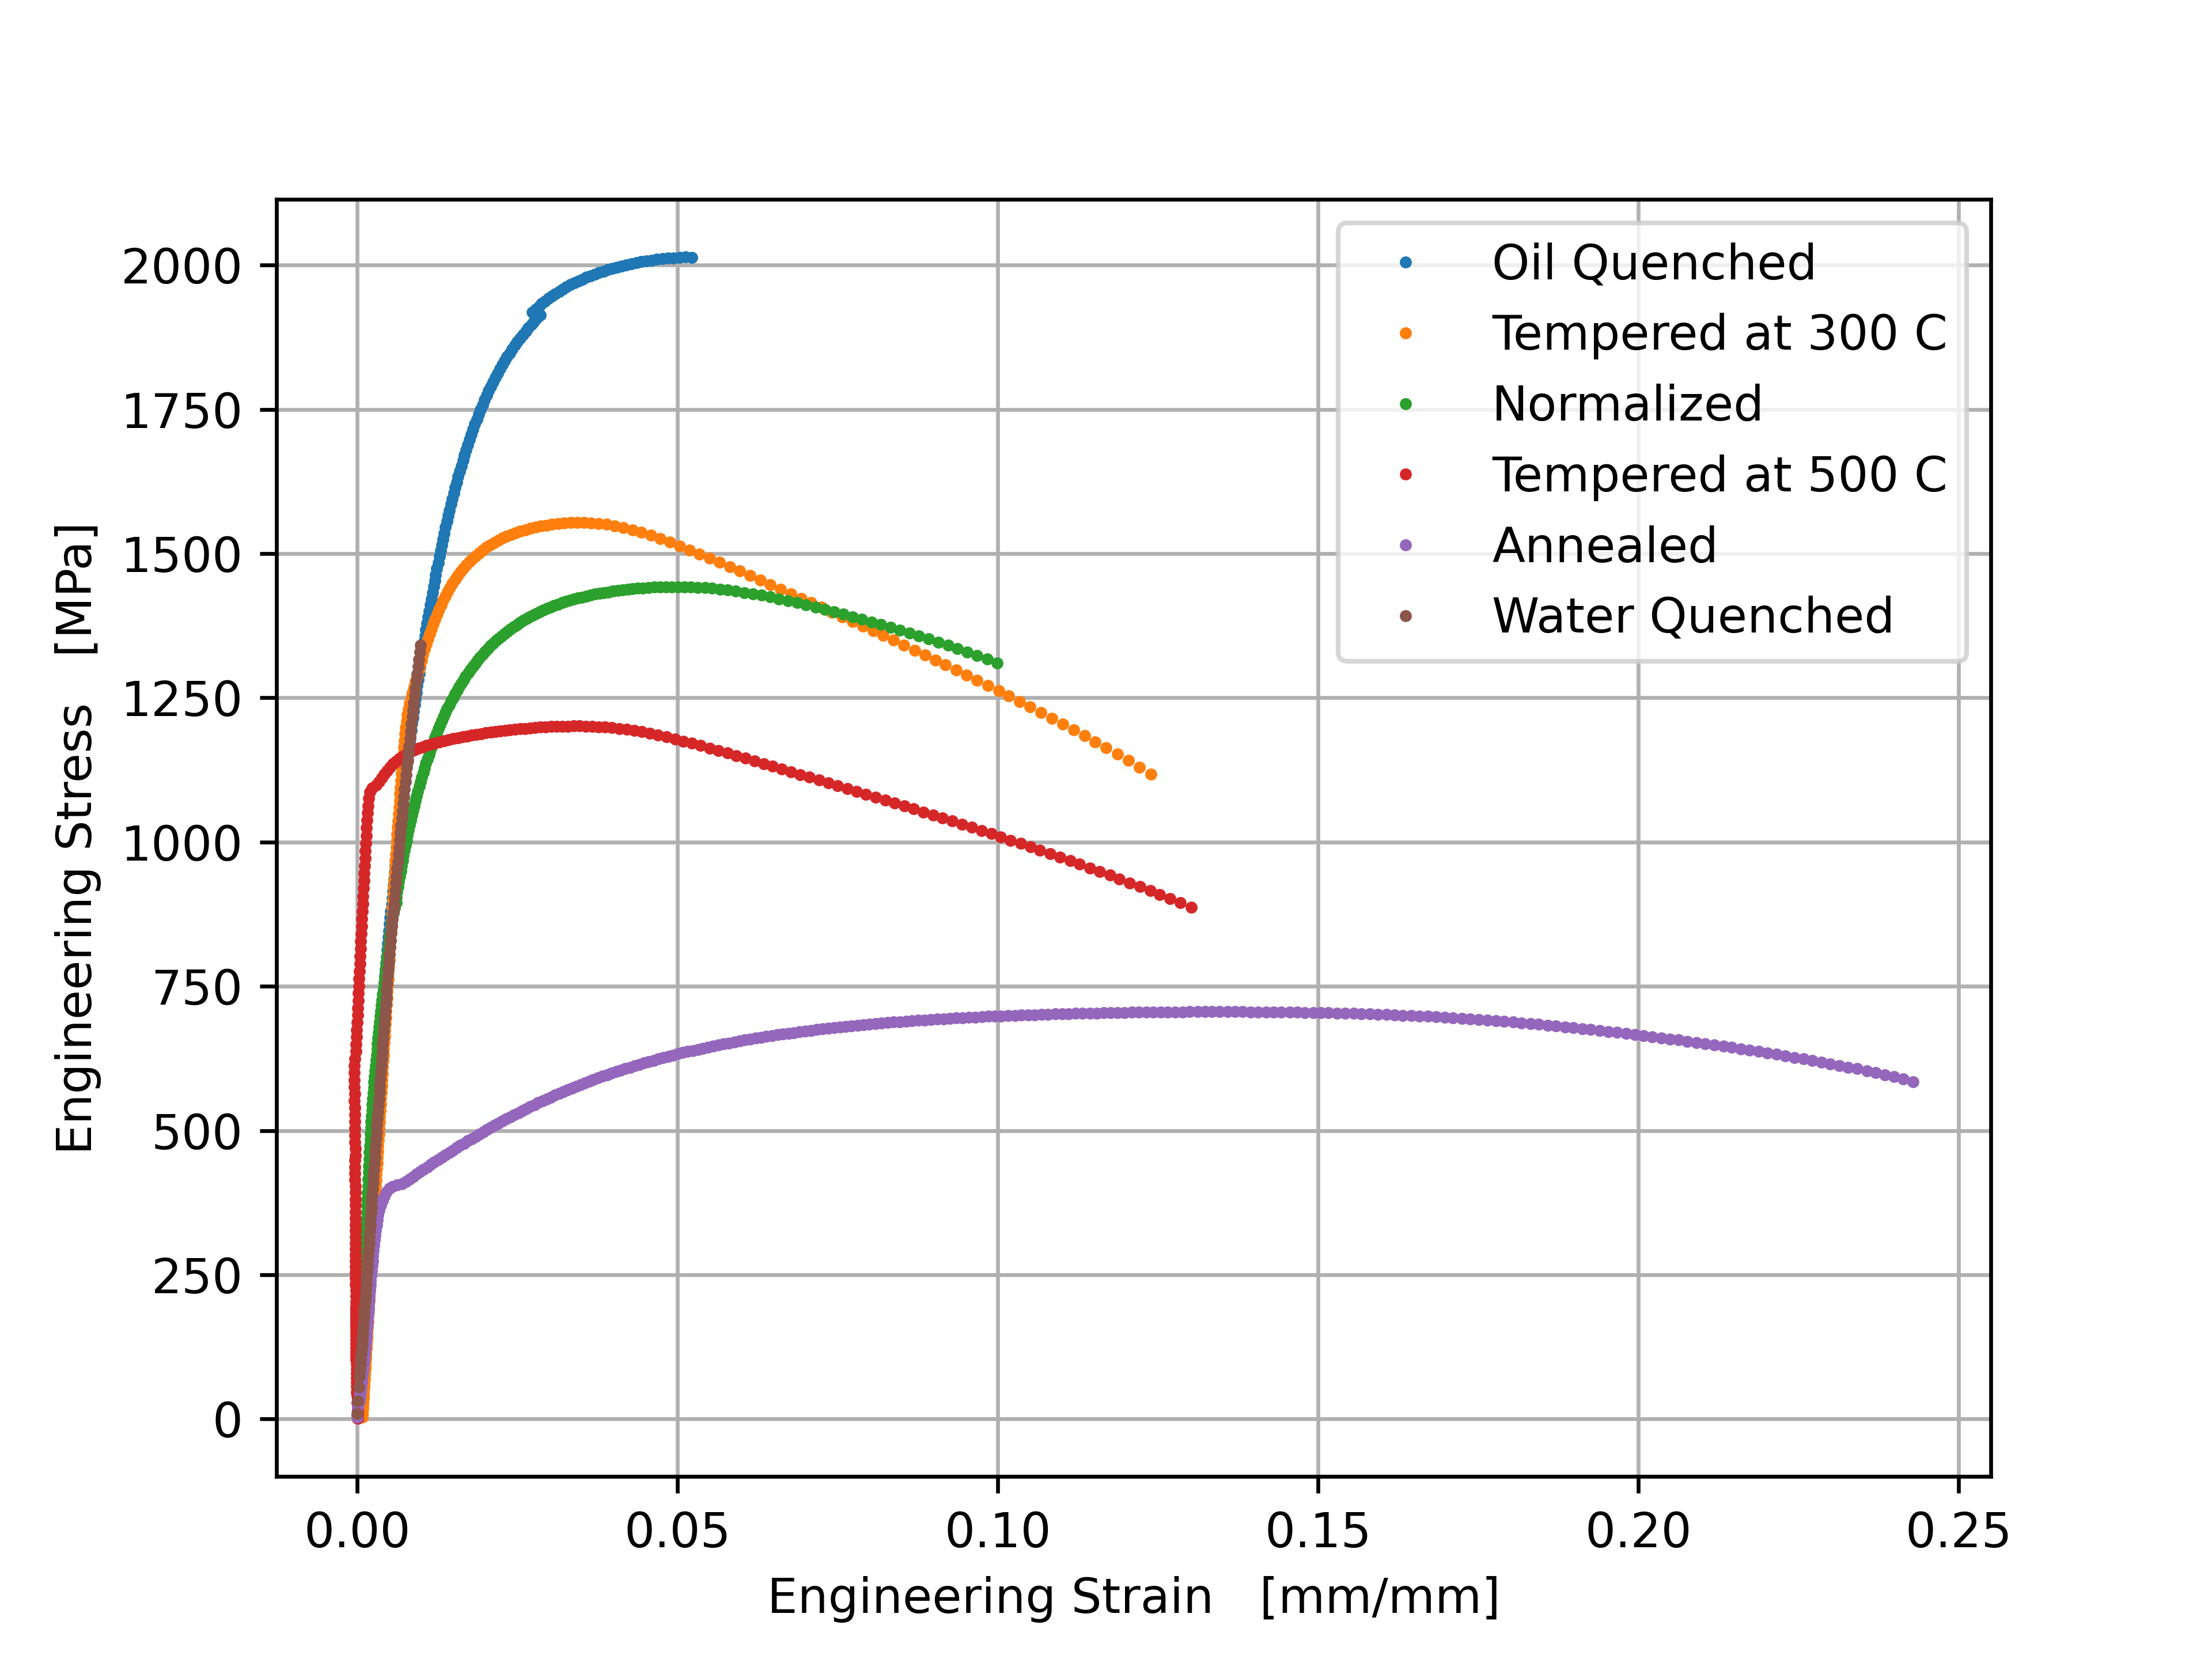
\includegraphics[width=0.5\linewidth]{Lab5/plots/q1_adjusted.png}
    \caption{Engineering Stress-Strain curves of select materials}
    \label{fig:q1-all}
\end{figure}

Next, from Fig. \ref{fig:q1-all} we found the elastic modulus, the yield strength, the ultimate strength, the toughness, percent elongation, and Brinnel hardness for each specimen. To not have an overly wide table, the specimen names were abbreviated but follow the same order as in the legend of Fig. \ref{fig:q1-all}. The Brinnel hardness values were determined via the conversionary equation, Eq. \ref{eq:rc2br}, from our measured HRC values. The yield strengths were determined via the 0.2 \% offset methodology.

\begin{table}[!h!]
    \centering
    \renewcommand{\arraystretch}{1.5}
    \caption{Select material properties of each specimen tested}
    \begin{tabular}{|c|c|c|c|c|c|c|}
        \toprule
        \hline
        \textbf{Material} & \textbf{OQ} & \textbf{Temp. 300} & \textbf{Norm.} & \textbf{Temp. 500} & \textbf{An.} & \textbf{WQ} \\ 
        \midrule
        \hline 
        \textbf{Youngs Modulus [GPa]} & 197.065 & 186.829 & 205.729 & 227.167 & 111.797 & 161.711 \\ 
        \hline 
        \textbf{Yield Strength} & 1138.428 & 1269.068 & 931.842 & 1148.958 & 402.874 & 1341.104 \\ 
        \hline 
        \textbf{Ultimate Strength} & 2013.803 & 1553.692 & 1442.464 & 1201.172 & 705.882 & 1341.104 \\ 
        \hline 
        \textbf{Toughness} & 86.562 & 166.139 & 131.696 & 142.251 & 155.675 & 7.386 \\ 
        \hline 
        \textbf{Percent Elongation} & 5.22 & 12.392 & 9.992 & 13.061 & 24.284 & 0.991 \\ 
        \hline 
        \textbf{Brinnel Hardness} & 264.692 & 309.453 & 238.109 & 247.905 & 1206.654 & 353.671 \\ 
        \hline 
    \end{tabular}
    \label{tab:q2}
\end{table}

Next, from these tabulated values we can determine a correlation between the  the ultimate strength and Brinnel hardness of each specimen, presented in Fig. \ref{fig:q4}. The linear-regression was performed with the use of \texttt{scipy.stats.linregress}. Next, again from Table \ref{tab:q2}, we determined the correlations between the ultimate strength, the yield strength, the elastic modulus, and the percent of elongation and the Brinnel hardness for specifically the oil quenched and the oil quenched then tempered specimens.

\begin{figure}[!h!]
    \centering
    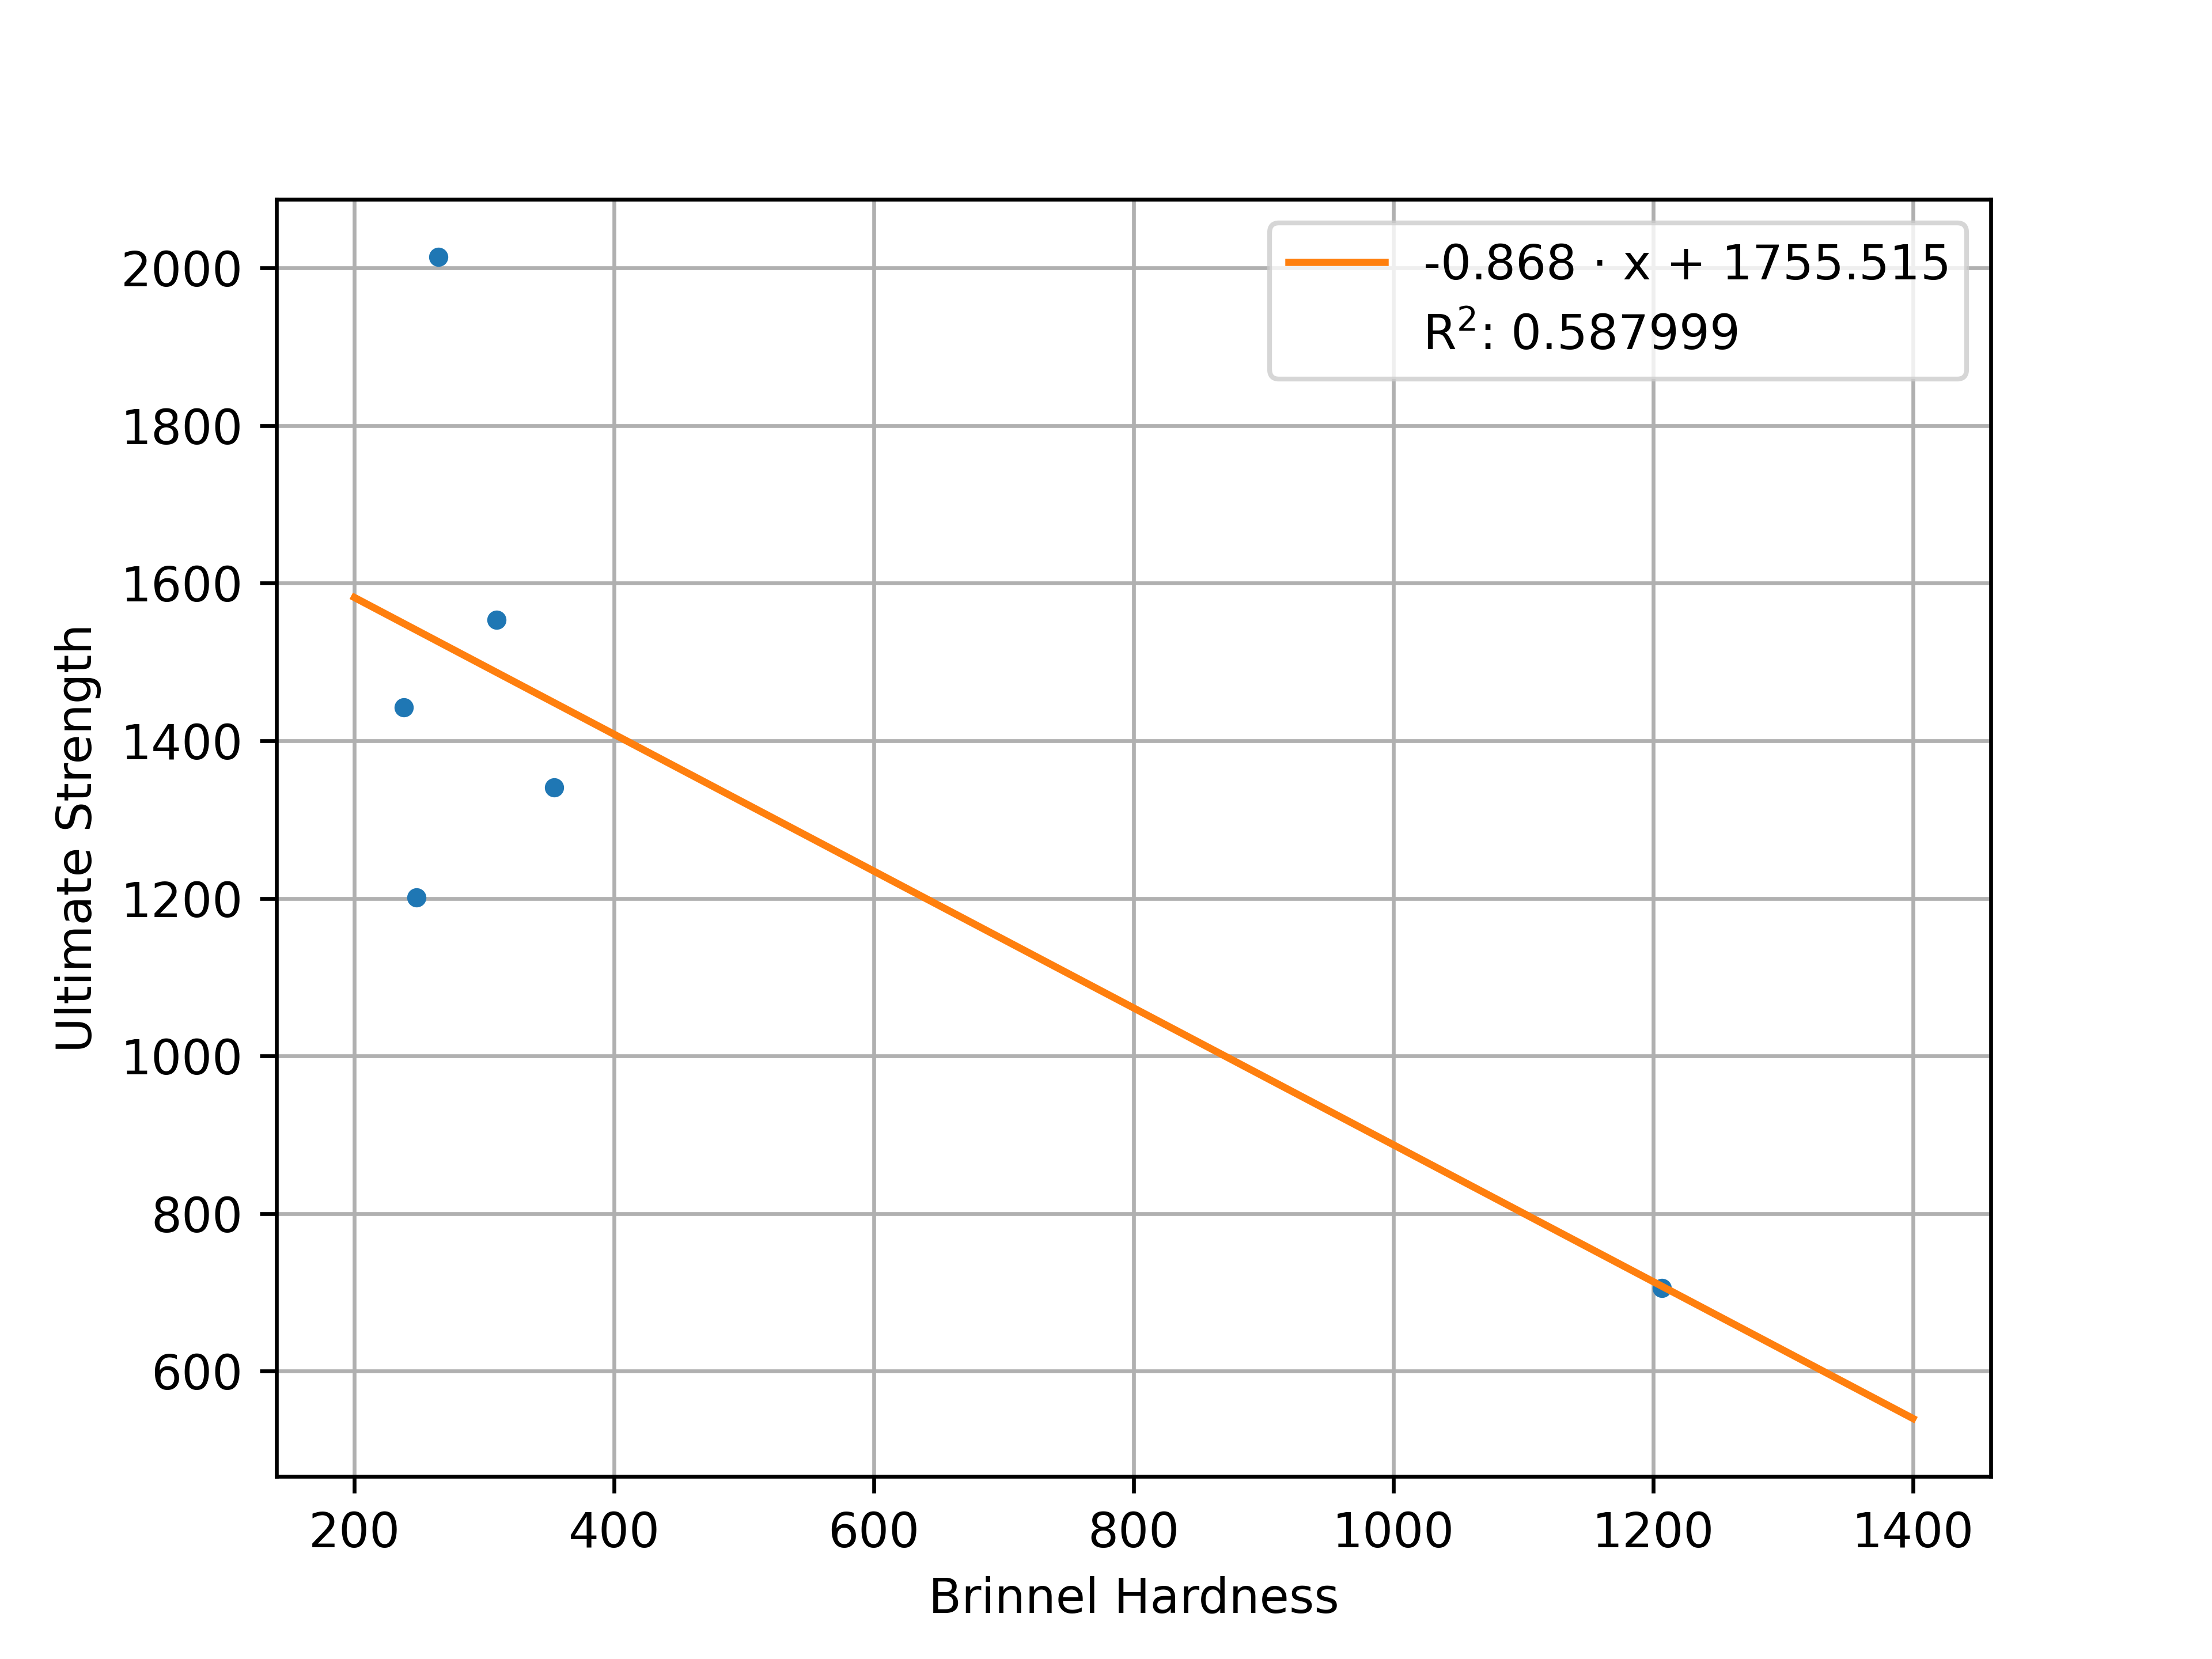
\includegraphics[width=0.5\linewidth]{plots/q4.png}
    \caption{Correlation of $\sigma_{UTS}$ to BHN for all specimens}
    \label{fig:q4}
\end{figure}


\begin{figure}[!h!]
\begin{minipage}[b]{.5\linewidth}
    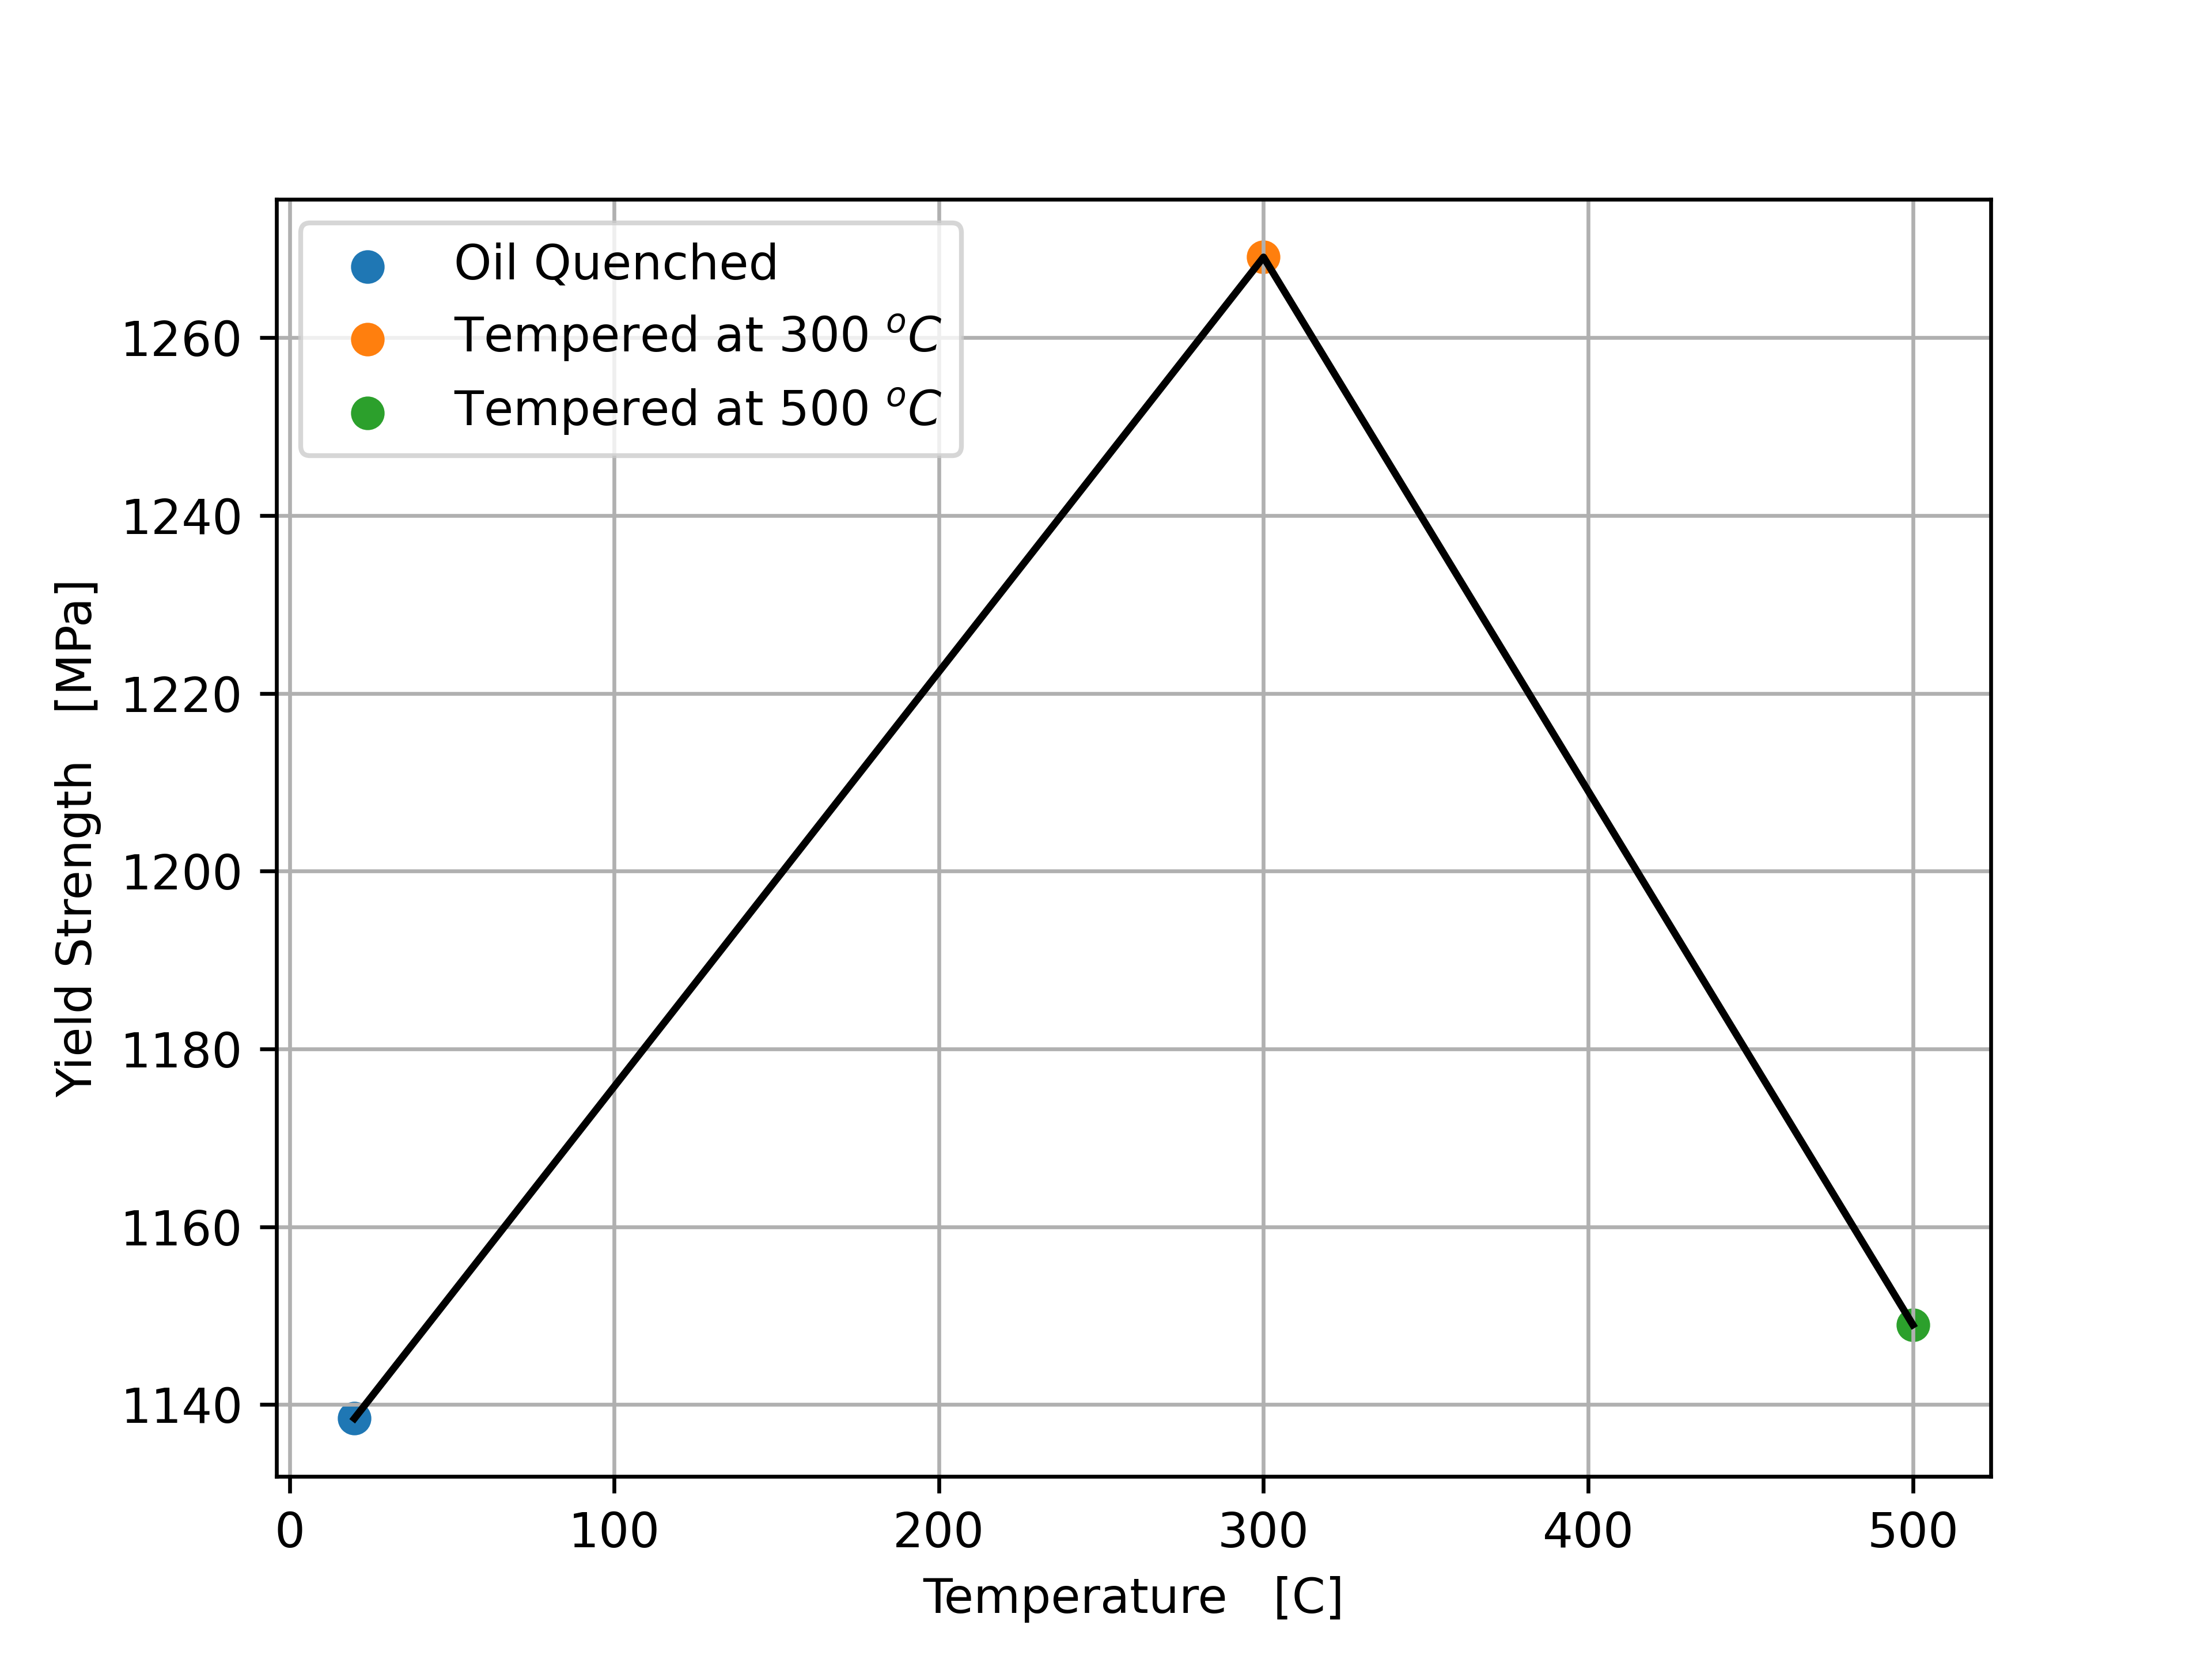
\includegraphics[width=\linewidth]{plots/q6_offset.png}
    \caption{Correlation of $\sigma_y$ to BHN}
    \label{fig:q6-yield}
    \vspace{4ex}
\end{minipage}
\begin{minipage}[b]{.5\linewidth}
    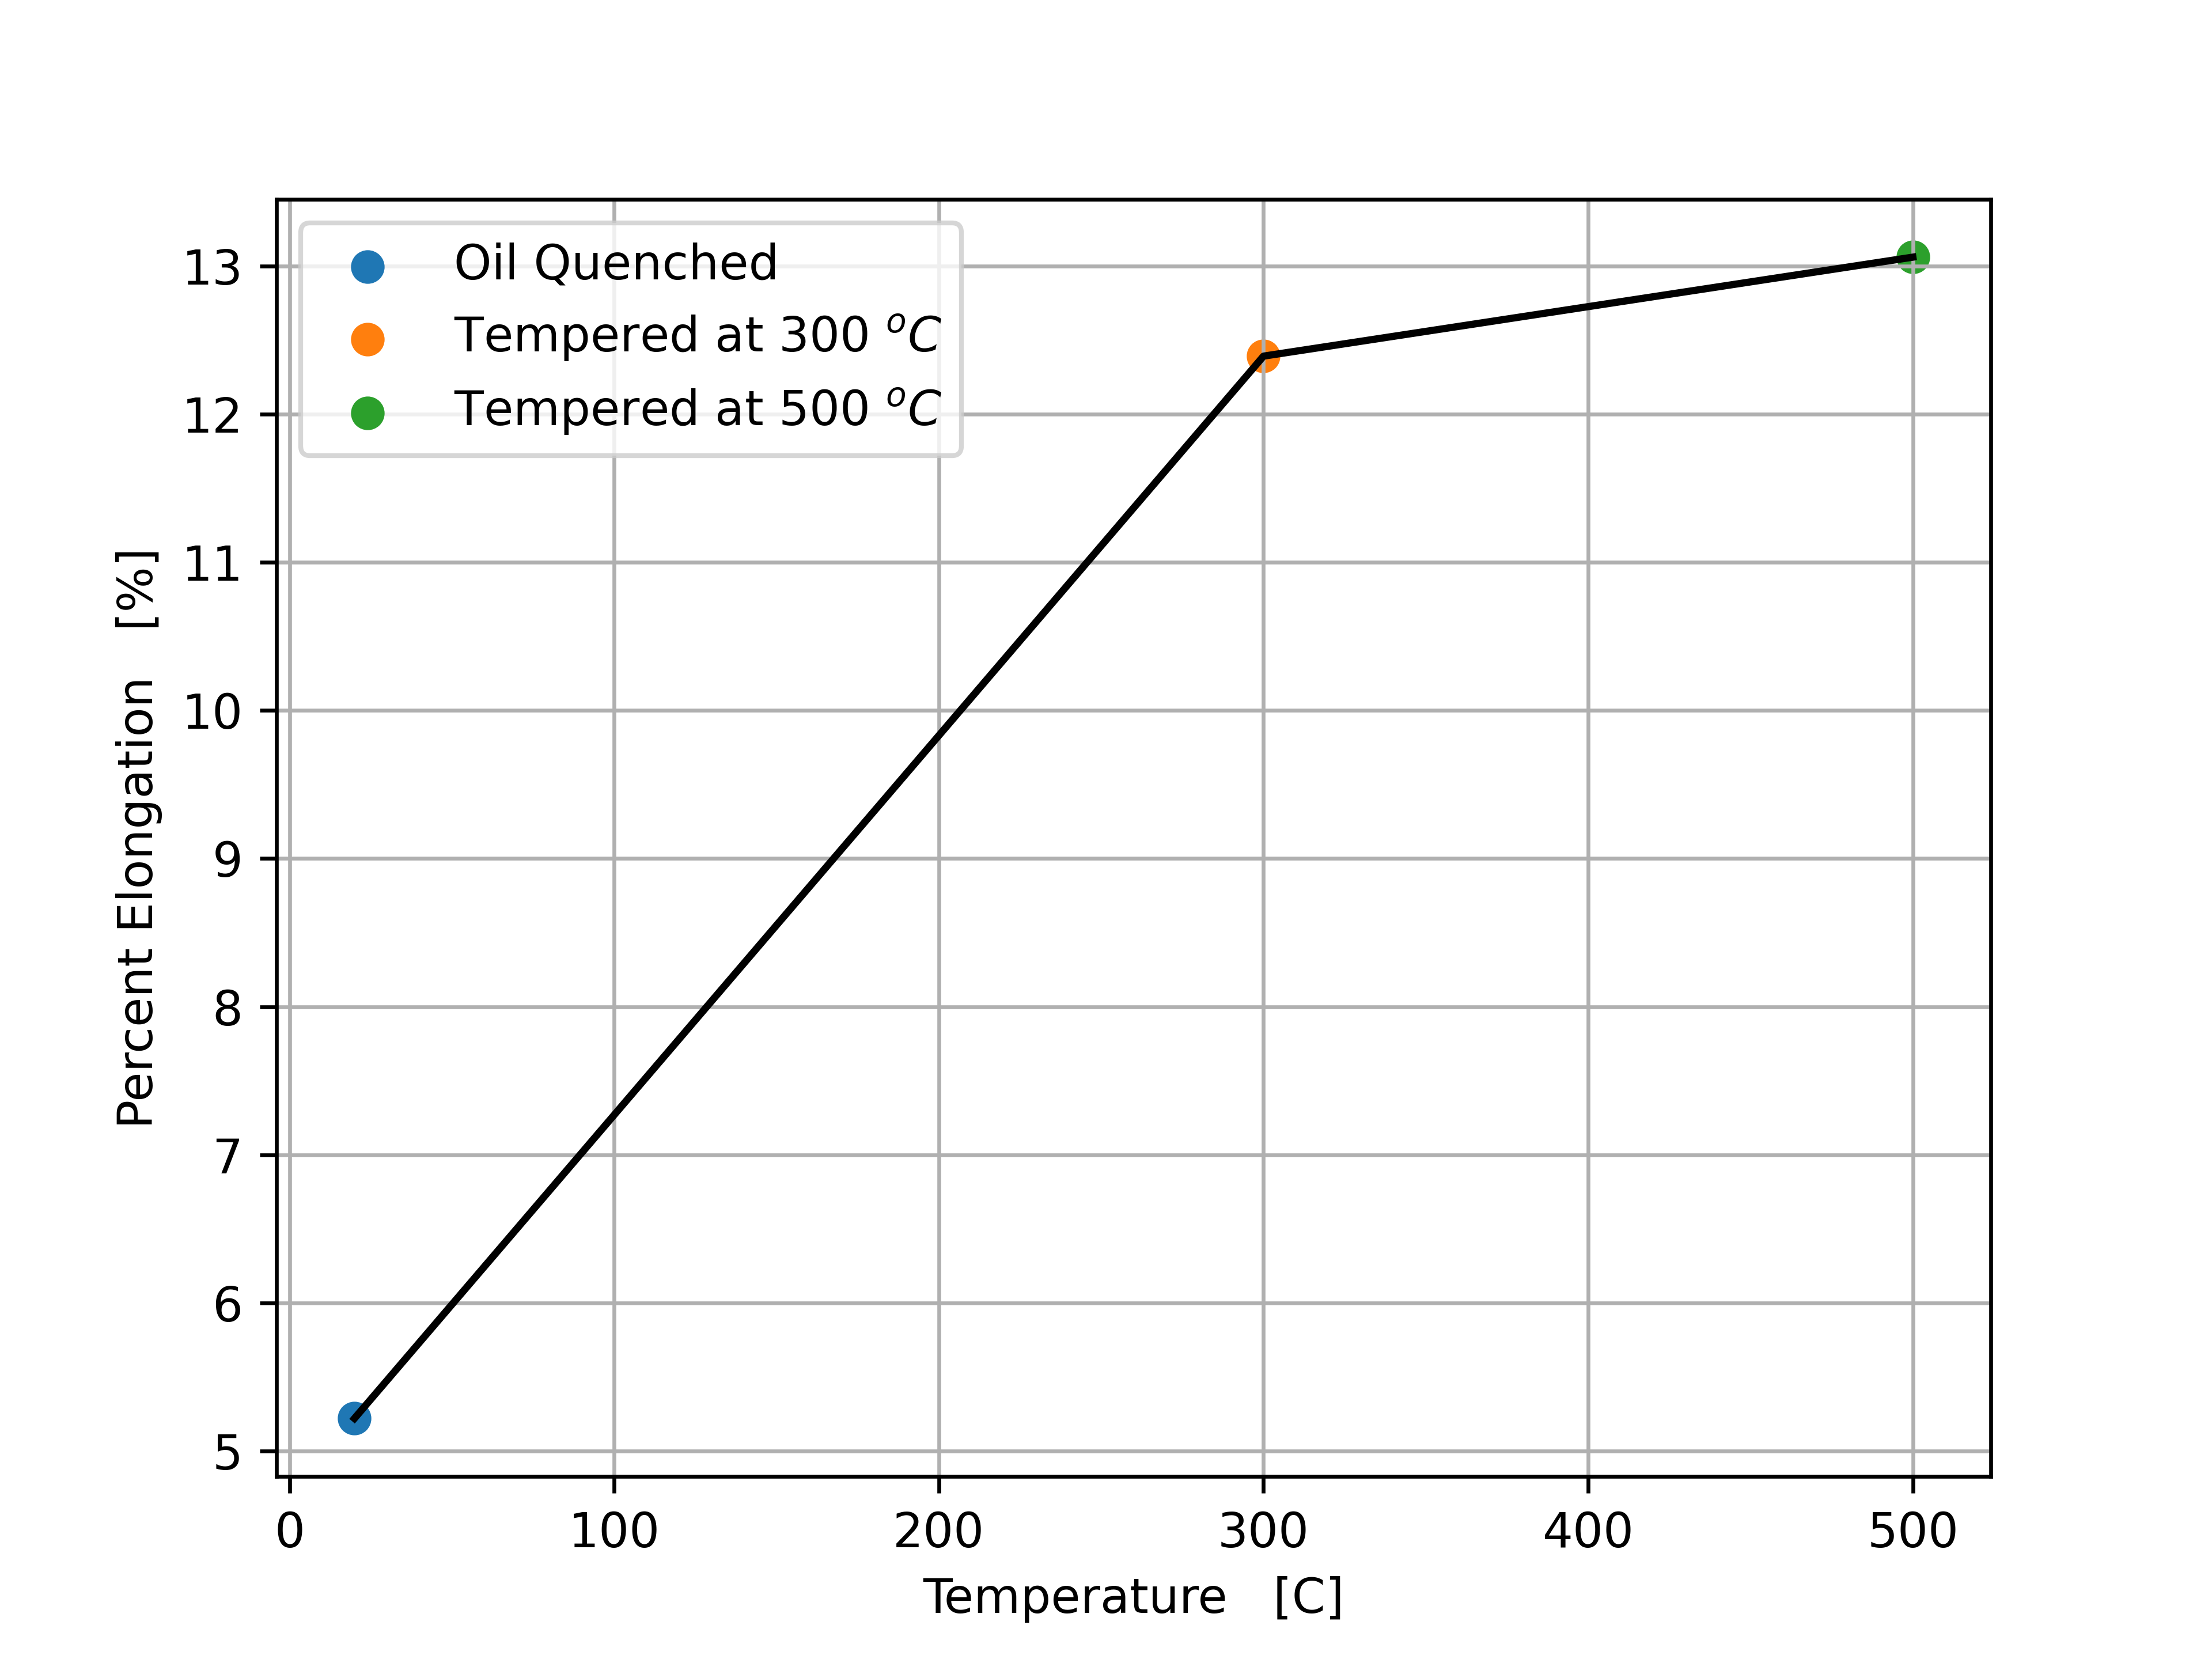
\includegraphics[width=\linewidth]{plots/q6_per_elong.png}
    \caption{Correlation of $\%_{elongation}$ to BHN}
    \label{fig:q6-perelong}
    \vspace{4ex}
\end{minipage}
\begin{minipage}[b]{.5\linewidth}
    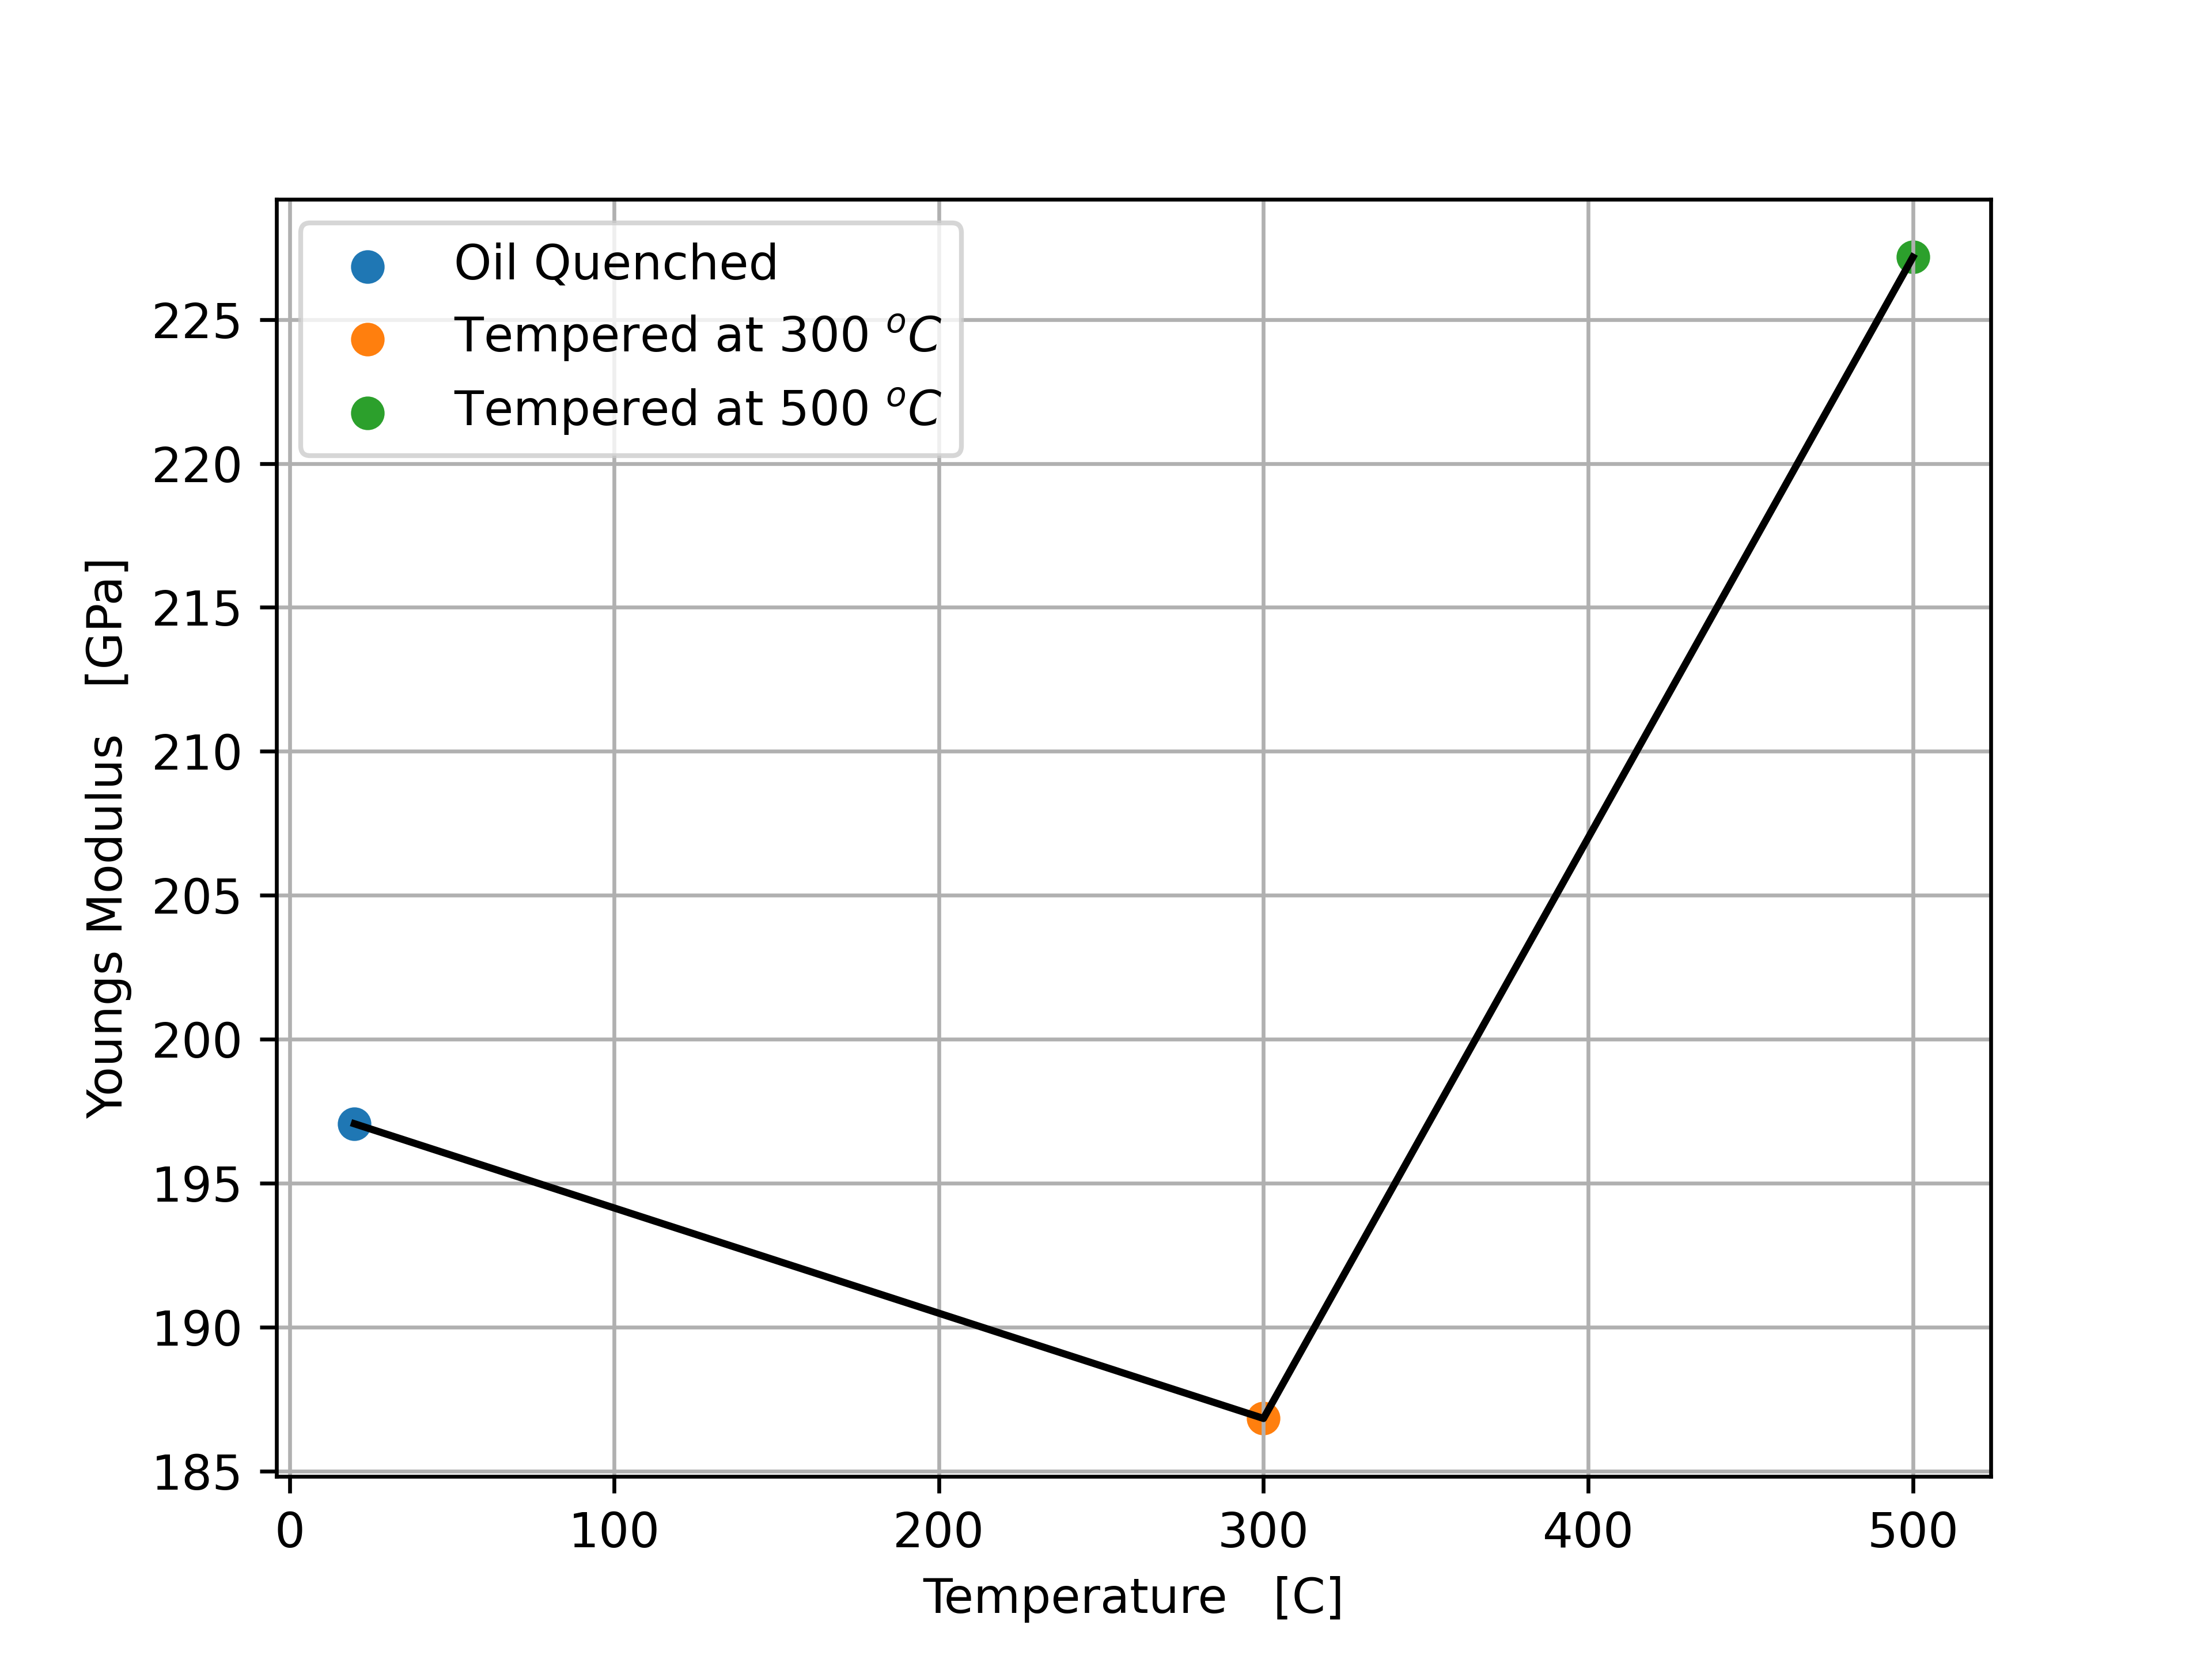
\includegraphics[width=\linewidth]{plots/q6_youngs.png}
    \caption{Correlation of $E$ to BHN}
    \label{fig:q6-youngs}
    \vspace{4ex}
\end{minipage}
\begin{minipage}[b]{.5\linewidth}
    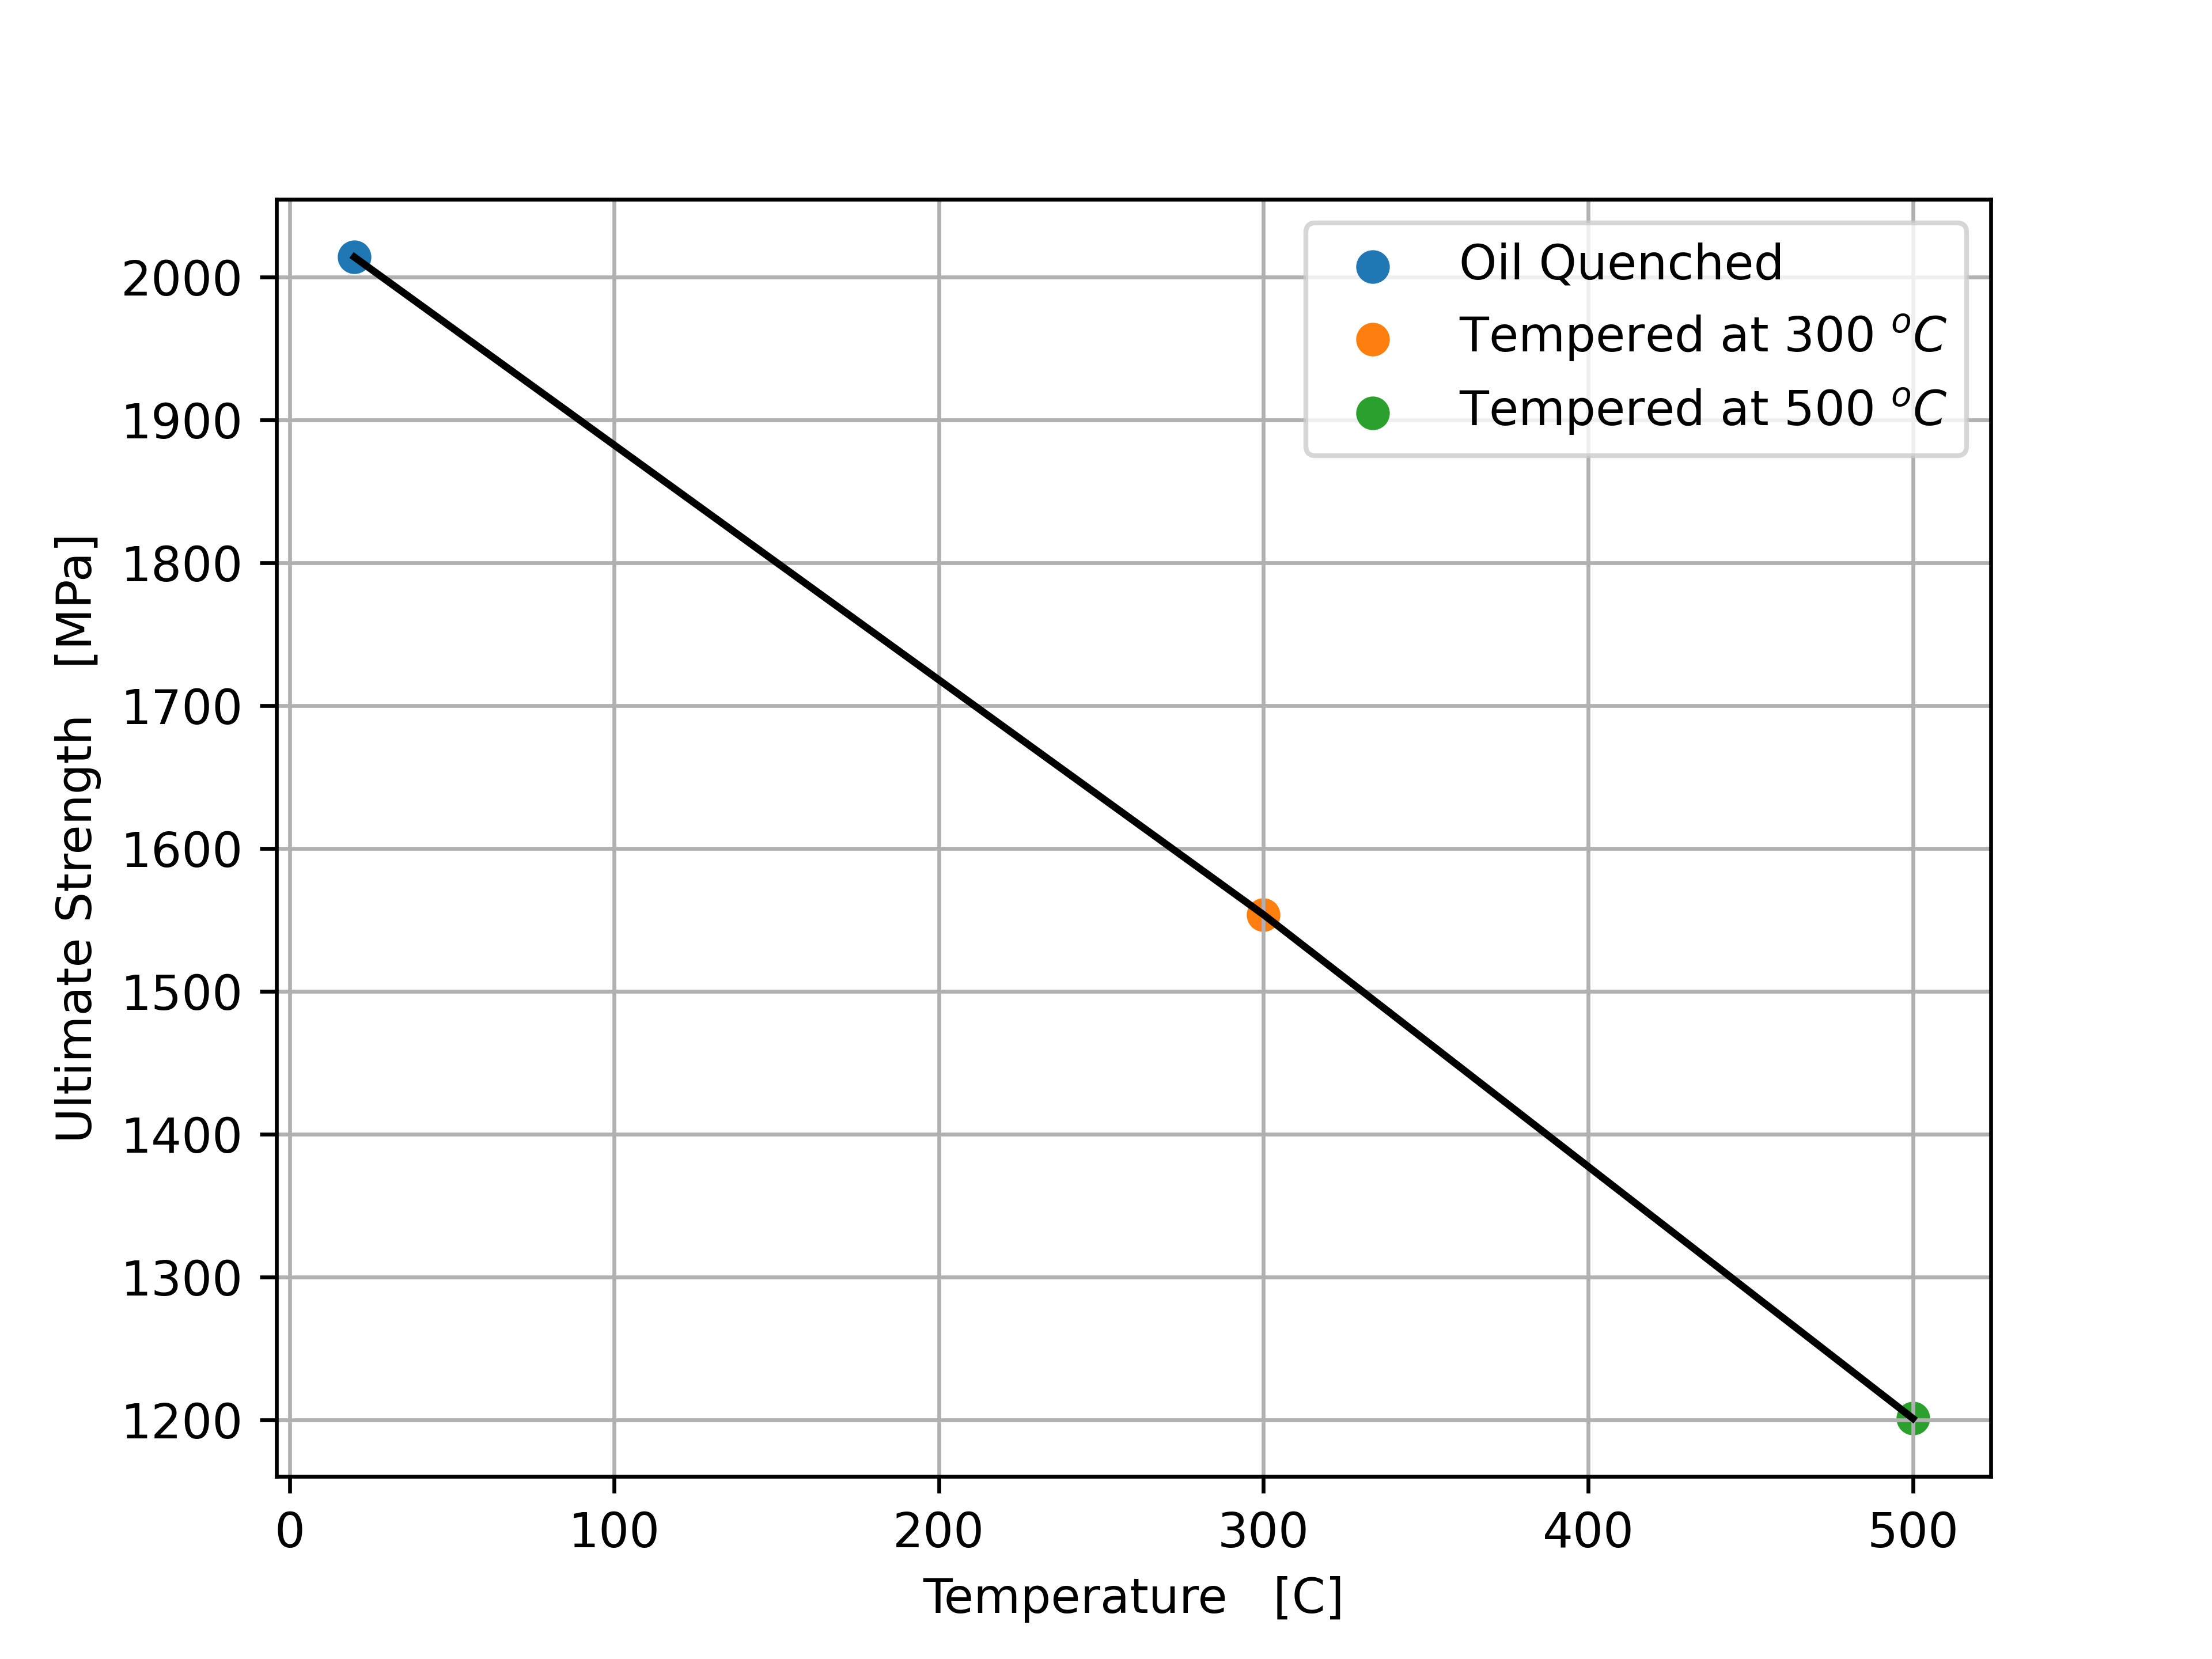
\includegraphics[width=\linewidth]{plots/q6_uts.png}
    \caption{Correlation of $\sigma_{UTS}$ to BHN}
    \label{fig:q6-uts}
    \vspace{4ex}
\end{minipage}
\end{figure}
\newpage
\section{Analysis of Discussion and Results}
To begin, our true-uncorrected data is rather lugubrious. This is due to mal-practice in loading of specimens, and so many of our trials either began with negative strains or started at 0 and then went negative prior to going positive. To amend these poor results, we chopped off the objectively incorrect data points that were obviously produced from incorrect loading, and then performed our data processing on the resulting datasets. For example, our normalized stress strain curve:

\begin{figure}[!h!]
    \centering
    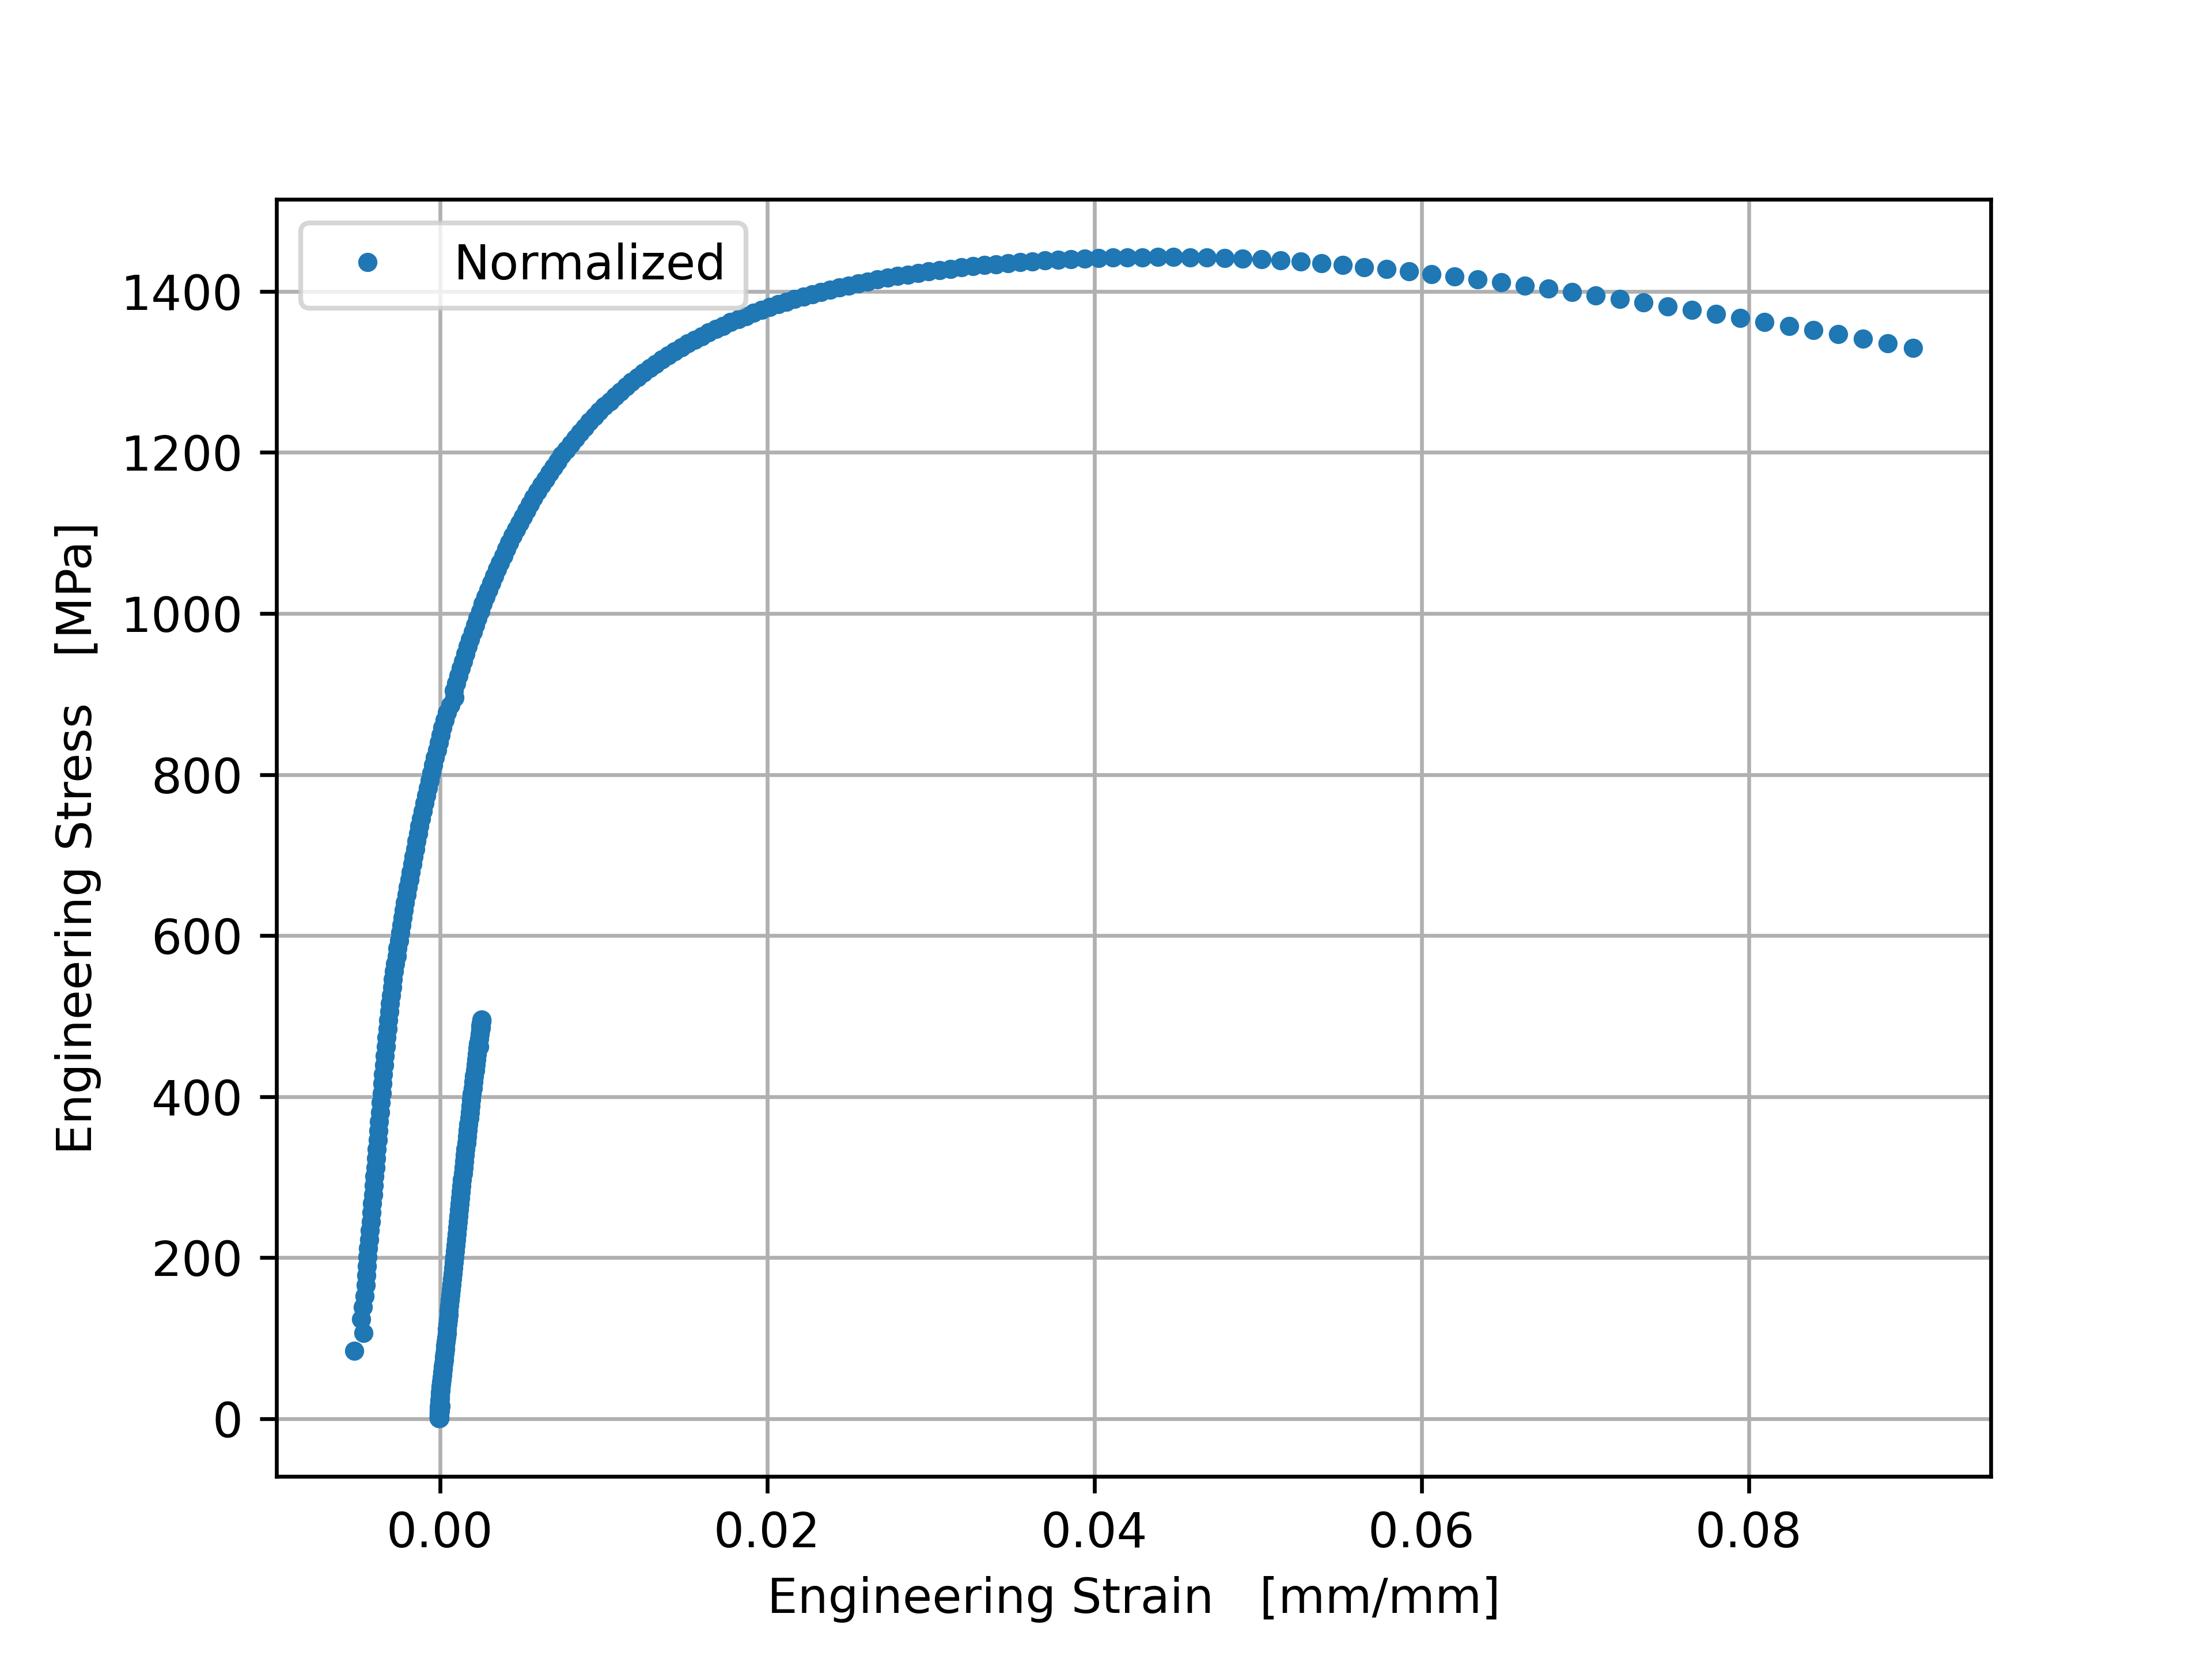
\includegraphics[width=0.5\linewidth]{plots/bs_plot.png}
    \caption{Normalized Stress-Strain curve, pre-adjusting}
    \label{fig:bs-plot}
\end{figure}

To fix this data set, we chopped the initial loading phase from the data set, removing the strong discontinuity. 

To continue, another strong source of error was in finding the Brinnel hardness of the annealed sample. This is due to the invalidity of application of the equation we utilized to convert between Rockwell C and Brinnel for this specimen. Similarly, when determining the toughness of the water quenched sample, because our mechanism in determining yield strength resulted in equivalent fracture point and yield strengths, the numerical integration was invalid. To obtain a non-zero value we integrated from 0 to the fracture point. We recognize this is invalid. 


\section{Answer to Questions}
To begin, we found and plotted the engineering stress-strain curves of various heat treatment methods enacted upon 4340 specimens. We investigated basic water quenched, basic oil quenched, annealed, normalized, oil quenched then tempered at 300 $^oC$, and oil quenched then tempered at 500 $^oC$. These curves are presented in Fig. \ref{fig:q1-all}.

Next, we found the elastic modulus, yield strength, ultimate tensile strength, toughness, percent elongation, and brinnel hardness of each aforementioned specimen. These values are tabulated in Tab. \ref{tab:q2}. Various results stand out, namely the yield strength of the water quenched specimen and the hardness of the annealed specimen. For the water quenched specimen, unfortunately when utilizing the 0.2\% offset method to determine the yield strength, the offset linear line never intercepted with the stress-strain curve as the specimen failed prior to significant plastic deformation. Further, the Brinnel hardness value for the Annealed specimen is absurdly high. This is due to the Rockwell hardness being very large ---- 87.9 ---- and outside of the range of validity of our empirically derived conversion equation, Eq. \ref{eq:rc2br}.

Noticeably, the material properties for each specimen are starkly different despite all being 4340. This is due to the affect that heating and cooling have on the microstructure of materials. In 4340, the faster the specimen is cooled the more martensite is present, and the more brittle the specimen is. The strongest specimen, by far, was the standard oil quenched specimen. The hardest was the annealed specimen. The stiffest was the water quenched whereas the most ductile was the annealed specimen. Finally, the toughest was the oil quenched then tempered at 300 $^oC$.

We determined the relationship between the ultimate tensile strength and the Brinnel hardness of each specimen, presented in Fig. \ref{fig:q4}. Our linear regression yielded a less than optimal correlation ---- only 0.588. Despite the poor fit, we do expect an inverse relationship between hardness and ultimate strength. We expect this as the harder a material is, the tougher we expect, and thus the less ductile. This is a gross over-simplification on the relationship between hardness and strength, but is sufficient for comparison's sake. 

The heat treatment that results in potential surface flaws is water quenching. This is due to the rapidity in cooling due to the high thermal conductivity of water. This rapid cooling is so strong and fast that it exerts huge thermal stresses upon the specimen, where portions of the surface experience rapid thermal de-expansion, potentially yielding cracks that can propagate through the material during tensile load. In fact, this was present in our water quenched specimen, where the specimen failed prior to non-negligible plastic deformation. 

Next, we determined the relationships between ultimate strength, yield strength, elastic modulus, and percent elongation versus tempering temperature for all of the oil quenched specimens. These specimens are the simple oil quenched, the oil quenched then tempered at 300 $^oC$, and the oil quenched then tempered at 500 $^oC$. These relationships are presented in Figs. \ref{fig:q6-yield} - \ref{fig:q6-uts}.



7. In your report, include micrographs of any three of the heat treatments that you were shown in the lab.
Label the phases. Compare and contrast the resulting microstructures.




8. Using the heat treatment micrographs from lab, describe the microstructure that is present in each case,
stating what phases are present and in (approximately) what amounts. When possible, compare the
relative phase amounts to what you expect from the equilibrium iron-carbon phase diagram.




9. How does each microstructure arise from its heat treatment? Explain how material properties relate to
these heat treatment procedures as well as the microstructures (i.e. how does processing effect
microstructure effect properties?)




\section{Bibliography}

\end{document}